
\documentclass[a4paper,12pt]{scrbook}
\usepackage{amsmath,amssymb,amsthm}
\usepackage{fancyvrb}
\usepackage{parskip}
\usepackage{lastpage}
\usepackage{verbatim,boxedminipage,enumitem}
\usepackage{ifthen}
\usepackage{color,graphicx}
\usepackage{pgf}
\usepackage{longtable}
\usepackage{upquote}
%\usepackage[all]{xy}
\usepackage{tobiShell}
\usepackage{tikz}
\usetikzlibrary{automata}
\usetikzlibrary{arrows}
\usepackage{pgf,pgfarrows,pgfnodes}
\usepackage{pgfplots}
\usepackage{circuitikz}
\usetikzlibrary{circuits}
\usetikzlibrary{circuits.logic.US}
\usepackage{mymath}
\usepackage{python}
%------------------------------------------------------------------
% Verbatim for console window - single line frame, no line numbers
%------------------------------------------------------------------
\DefineVerbatimEnvironment%
 {console}{Verbatim}
 {frame=single}

%--------------------------------------------------------
% Remove the vertical spacing before and after Verbatim.
%--------------------------------------------------------
\usepackage{atbeginend}
\BeforeBegin{console}{\mbox{}\\ \begin{minipage}{\textwidth}\vspace{3pt}}
\AfterEnd{console}{\vspace{4pt} \end{minipage} \\ }

\begin{document}
\thispagestyle{empty}

\begin{center}
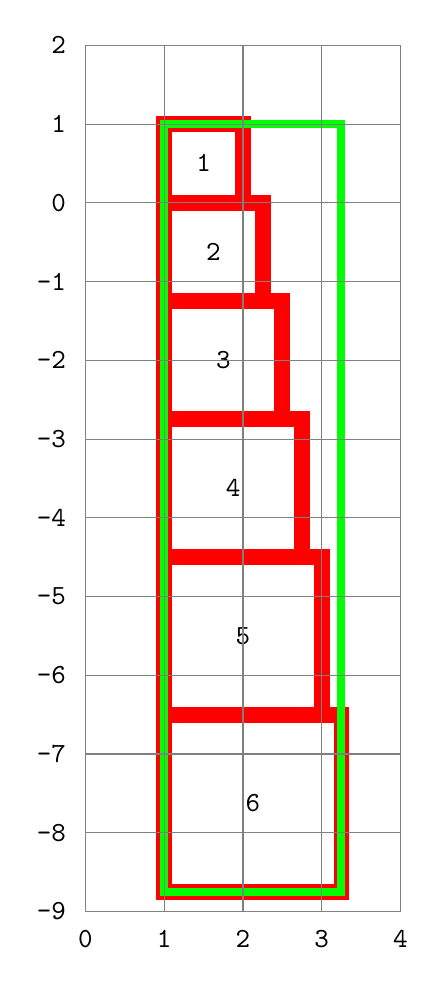
\begin{tikzpicture}

\draw (1.5, 0.5)
  node[draw, line width=0.2cm, , color=red,
       rounded corners=0cm, inner sep=0cm] {

\begin{minipage}[t][1.0cm]{1.0cm}
\mbox{}

\end{minipage}

};\draw (1.5, 0.5) node[color=black] {{\texttt{1}}};
\draw (1.625, -0.625)
  node[draw, line width=0.2cm, , color=red,
       rounded corners=0cm, inner sep=0cm] {

\begin{minipage}[t][1.25cm]{1.25cm}
\mbox{}

\end{minipage}

};\draw (1.625, -0.625) node[color=black] {{\texttt{2}}};
\draw (1.75, -2.0)
  node[draw, line width=0.2cm, , color=red,
       rounded corners=0cm, inner sep=0cm] {

\begin{minipage}[t][1.5cm]{1.5cm}
\mbox{}

\end{minipage}

};\draw (1.75, -2.0) node[color=black] {{\texttt{3}}};
\draw (1.875, -3.625)
  node[draw, line width=0.2cm, , color=red,
       rounded corners=0cm, inner sep=0cm] {

\begin{minipage}[t][1.75cm]{1.75cm}
\mbox{}

\end{minipage}

};\draw (1.875, -3.625) node[color=black] {{\texttt{4}}};
\draw (2.0, -5.5)
  node[draw, line width=0.2cm, , color=red,
       rounded corners=0cm, inner sep=0cm] {

\begin{minipage}[t][2.0cm]{2.0cm}
\mbox{}

\end{minipage}

};\draw (2.0, -5.5) node[color=black] {{\texttt{5}}};
\draw (2.125, -7.625)
  node[draw, line width=0.2cm, , color=red,
       rounded corners=0cm, inner sep=0cm] {

\begin{minipage}[t][2.25cm]{2.25cm}
\mbox{}

\end{minipage}

};\draw (2.125, -7.625) node[color=black] {{\texttt{6}}};
\draw (2.125, -3.875)
  node[draw, line width=0.1cm, , color=green,
       rounded corners=0cm, inner sep=0cm] {

\begin{minipage}[t][9.75cm]{2.25cm}
\mbox{}

\end{minipage}

};\draw[gray] (0.0,-9.0) -- (0.0,2);
\draw[gray] (1.0,-9.0) -- (1.0,2);
\draw[gray] (2.0,-9.0) -- (2.0,2);
\draw[gray] (3.0,-9.0) -- (3.0,2);
\draw[gray] (4.0,-9.0) -- (4.0,2);
\draw[gray] (0.0,-9.0) -- (4,-9.0);
\draw[gray] (0.0,-8.0) -- (4,-8.0);
\draw[gray] (0.0,-7.0) -- (4,-7.0);
\draw[gray] (0.0,-6.0) -- (4,-6.0);
\draw[gray] (0.0,-5.0) -- (4,-5.0);
\draw[gray] (0.0,-4.0) -- (4,-4.0);
\draw[gray] (0.0,-3.0) -- (4,-3.0);
\draw[gray] (0.0,-2.0) -- (4,-2.0);
\draw[gray] (0.0,-1.0) -- (4,-1.0);
\draw[gray] (0.0,0.0) -- (4,0.0);
\draw[gray] (0.0,1.0) -- (4,1.0);
\draw[gray] (0.0,2.0) -- (4,2.0);
\draw(0, -9) node [font=\ttfamily, label=below:{\texttt{0}}] {};
\draw(1, -9) node [font=\ttfamily, label=below:{\texttt{1}}] {};
\draw(2, -9) node [font=\ttfamily, label=below:{\texttt{2}}] {};
\draw(3, -9) node [font=\ttfamily, label=below:{\texttt{3}}] {};
\draw(4, -9) node [font=\ttfamily, label=below:{\texttt{4}}] {};
\draw(0, -9) node [font=\ttfamily, label=left:{\texttt{-9}}] {};
\draw(0, -8) node [font=\ttfamily, label=left:{\texttt{-8}}] {};
\draw(0, -7) node [font=\ttfamily, label=left:{\texttt{-7}}] {};
\draw(0, -6) node [font=\ttfamily, label=left:{\texttt{-6}}] {};
\draw(0, -5) node [font=\ttfamily, label=left:{\texttt{-5}}] {};
\draw(0, -4) node [font=\ttfamily, label=left:{\texttt{-4}}] {};
\draw(0, -3) node [font=\ttfamily, label=left:{\texttt{-3}}] {};
\draw(0, -2) node [font=\ttfamily, label=left:{\texttt{-2}}] {};
\draw(0, -1) node [font=\ttfamily, label=left:{\texttt{-1}}] {};
\draw(0, 0) node [font=\ttfamily, label=left:{\texttt{0}}] {};
\draw(0, 1) node [font=\ttfamily, label=left:{\texttt{1}}] {};
\draw(0, 2) node [font=\ttfamily, label=left:{\texttt{2}}] {};
\end{tikzpicture}

\end{center}

\end{document}
